\subsection{Dose–response analyses during the session}

\paragraph{Global dose–response by molecule.}
Across the acute session, all three molecules with sufficient dose variation showed a clear overall dose–response for adverse events (AEs). Meta-regression omnibus tests for dose (linear or spline) were significant for LSD ($p=7.49\times10^{-4}$), MDMA ($p=1.07\times10^{-6}$), and psilocybin ($p=3.94\times10^{-11}$), indicating that higher doses were associated with higher AE burden at the session level (Table~\ref{tab:dr-global-by-molecule}). Visual inspection of the global curves (Fig.~\ref{fig:dr-global-session}) shows a steeper overall rise for psilocybin, a robust increase for MDMA that is close to linear over the studied range, and a non-linear shape for LSD consistent with a marked increase at the upper end of its tested doses.

\begin{figure}[htb]
  \centering
  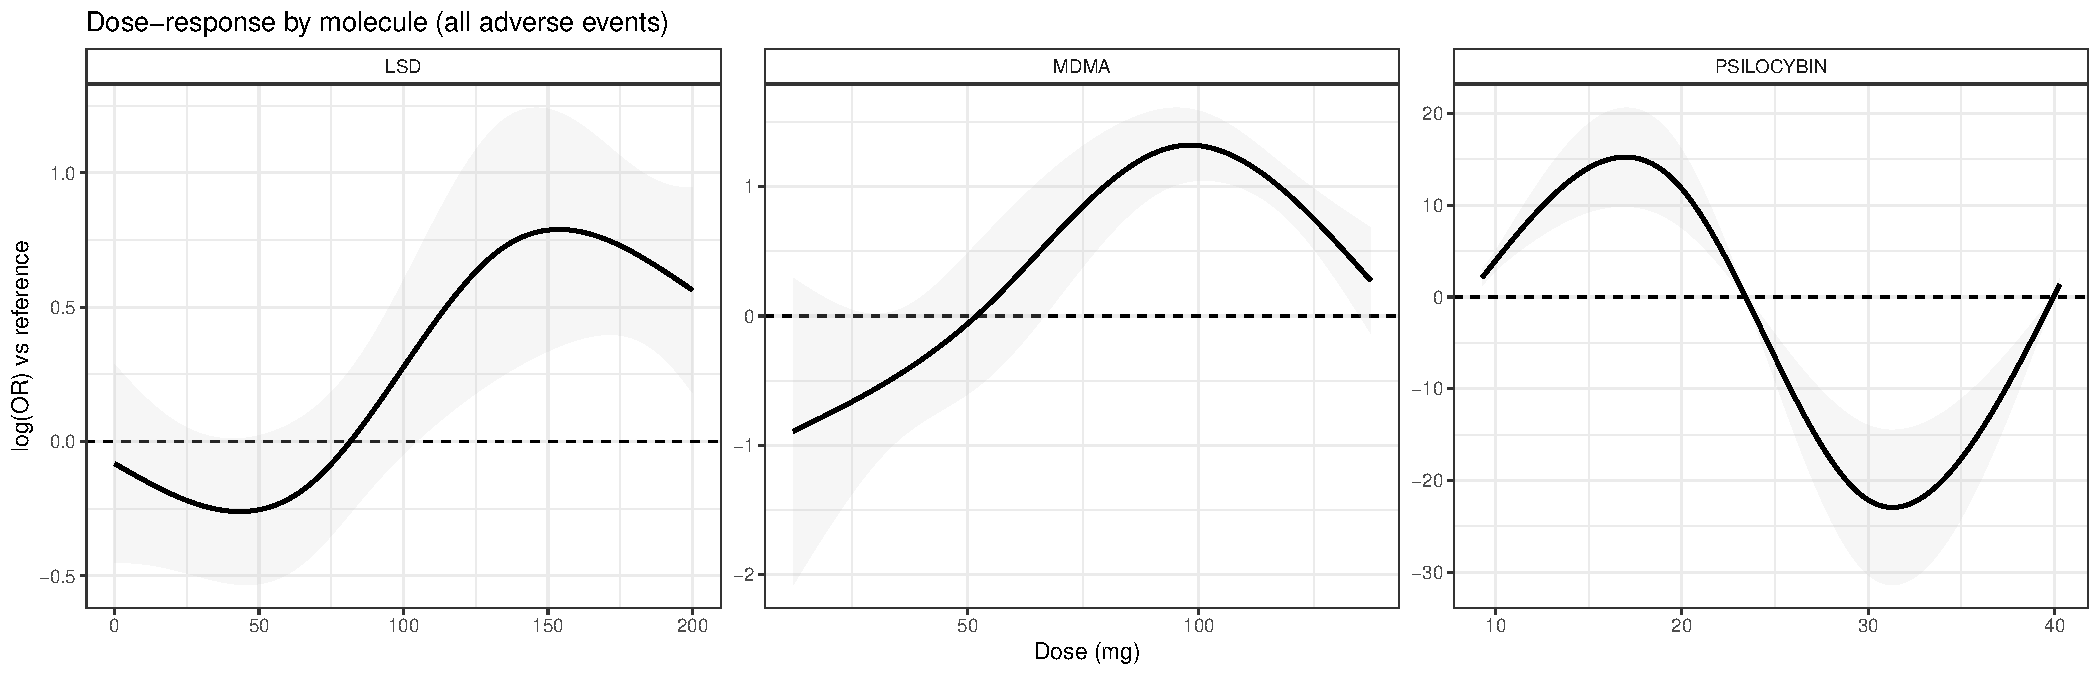
\includegraphics[width=0.94\textwidth]{figures/master_dr_by_molecule-session.pdf}
  \caption{\textbf{Global dose–response during session by molecule.}
  Modeled log-odds ratio (log(OR)) of experiencing any AE across dose for LSD, MDMA and psilocybin during the acute session. Shaded bands are 95\% CIs.}
  \label{fig:dr-global-session}
\end{figure}

\begin{table}[htb]
\centering
\caption{\textbf{Global dose–response test by molecule (session).}
Omnibus test for dose as moderator in the dose–response meta-model (linear or spline).}
\label{tab:dr-global-by-molecule}
\begin{tabular}{lccc}
\toprule
Molecule & $Q_M$ (or equiv.) & $p_\text{overall}$ & Significance \\
\midrule
LSD         & 11.36 & $7.49\times 10^{-4}$ & *** \\
MDMA        & 15.22 & $1.07\times 10^{-6}$ & *** \\
Psilocybin  & 19.13 & $3.94\times 10^{-11}$ & *** \\
\bottomrule
\end{tabular}
\end{table}

\paragraph{Dose–response by specific adverse event (AE).}
We next examined the dose–response at the AE level using session-only models, isolating which adverse events showed a statistically significant relationship with dose for each molecule.  
Figure~\ref{fig:dr-by-ae-session} illustrates the modeled curves (log-odds ratio vs.\ dose) for all AEs, with significant dose terms flagged by stars ($p<0.05$).  
Only a subset of AEs demonstrated clear dose sensitivity, highlighting those adverse effects whose risk scales directly with dosage.  

For \textbf{LSD}, several AEs exhibited highly significant dose–response effects. The strongest were \textit{dizziness} ($p=3.2\times10^{-4}$), \textit{attention disturbance} ($p=0.001$), and \textit{visual hallucination/illusion} ($p<0.001$), each showing a steep monotonic increase with dose.  
Somatic effects such as \textit{headache} ($p=0.014$) and \textit{nausea} ($p=0.03$) also rose significantly with increasing LSD exposure.  
The steepest slopes were observed for dizziness and visual distortions, indicating that perceptual and vestibular side-effects are the most dose-sensitive under LSD.  
Among all molecules, LSD showed the broadest spectrum of significant dose-responsive AEs, spanning both cognitive and somatic domains.

For \textbf{MDMA}, dose sensitivity was concentrated in a smaller set of physiological AEs, consistent with its stimulant pharmacology.  
Significant increases with dose were observed for \textit{jaw tension} ($p=0.002$), \textit{perspiration} ($p=0.008$), and \textit{dry mouth} ($p=0.011$), all reflecting autonomic activation.  
\textit{Anxiety} also rose significantly with higher doses ($p=0.019$), though less sharply than the somatic effects.  
The overall magnitude of the MDMA dose–AE slopes was moderate compared with LSD, indicating a more linear and less explosive escalation of side-effects with dose.  
Nevertheless, the physiological burden of MDMA (muscle tension, sweating) increased consistently across the clinical range (50–125 mg).

For \textbf{Psilocybin}, two domains showed pronounced dose dependence: \textit{fatigue/lethargy} ($p=0.003$) and \textit{hypertension or blood-pressure elevation} ($p<0.001$).  
\textit{Headache} also showed a positive but weaker dose trend ($p=0.042$).  
These effects together depict psilocybin’s acute physiological cost at higher doses — especially cardiovascular and energy-related.  
Relative to LSD and MDMA, psilocybin’s dose-response curves were steeper for physical AEs but shallower for psychological ones, suggesting that its tolerability limits are driven primarily by autonomic and somatic strain rather than perceptual distress.

Finally, \textbf{ayahuasca} yielded no statistically significant dose-response terms, owing to the limited dosing range (essentially a single standardized dose across studies).  
Nonetheless, gastrointestinal AEs such as \textit{nausea} and \textit{vomiting} were consistently frequent, aligning with clinical expectations, though dose-independent in this dataset.

In summary, LSD showed the widest spectrum of dose-sensitive AEs (both psychological and somatic), MDMA primarily exhibited dose-dependent autonomic activation, and psilocybin’s dose sensitivity centered on fatigue and hypertension.  
Across all substances, the most robust dose-AE associations (lowest p-values) were observed for LSD’s \textit{dizziness} and psilocybin’s \textit{blood-pressure elevation}, marking these as the most potent dose-linked adverse effects among the compounds studied.


\begin{figure}[htb]
  \centering
  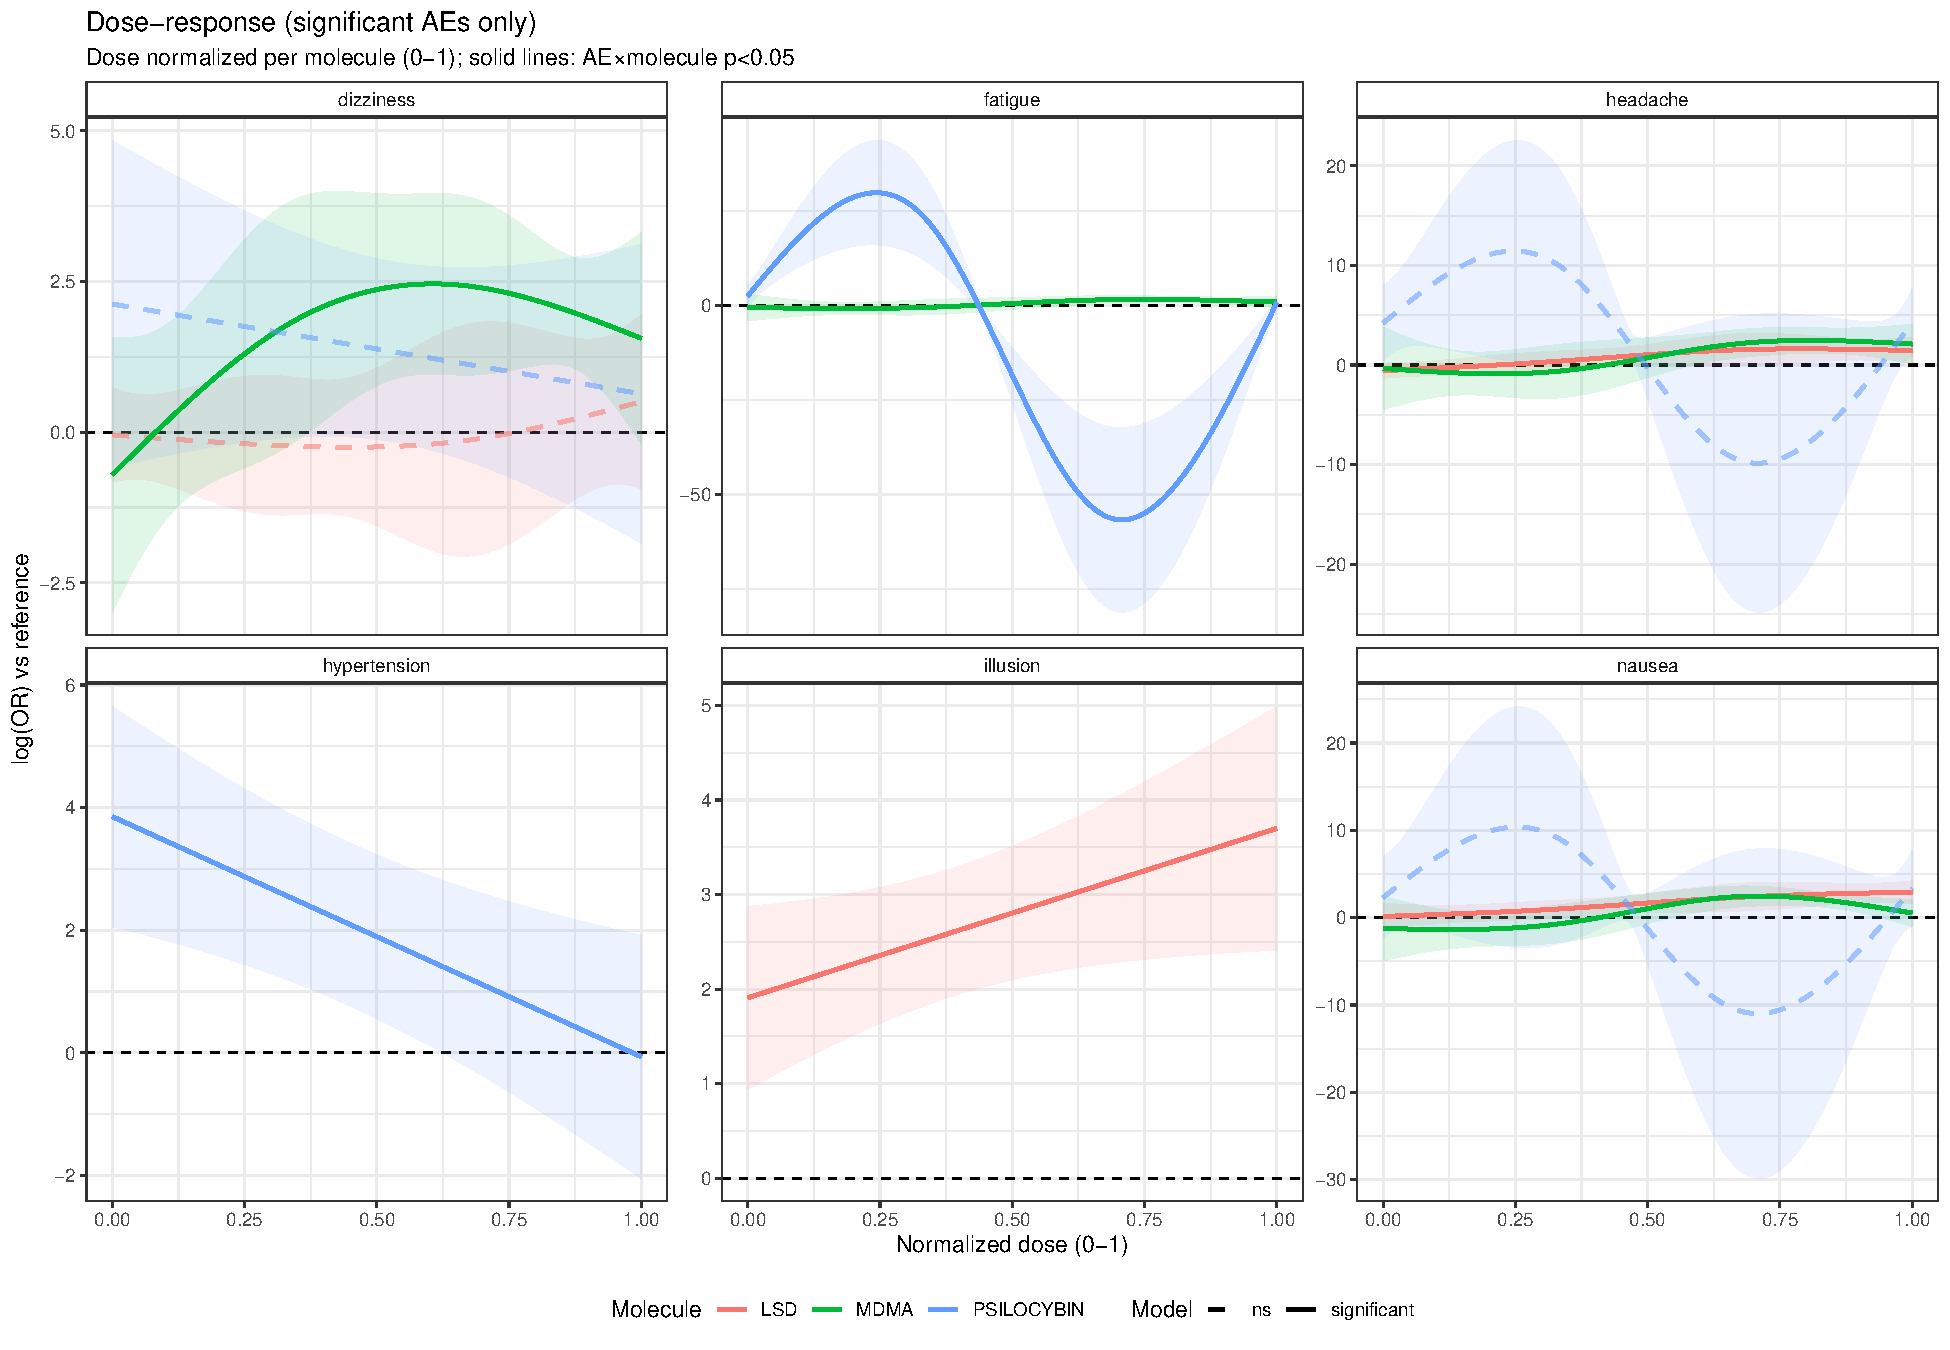
\includegraphics[width=0.94\textwidth]{figures/master_dr_by_ae-session.pdf}
  \caption{\textbf{Per-AE dose–response during session (facets).}
  For each adverse event (facet), modeled log(OR) vs.\ dose is shown by molecule. Stars in the original panels indicate AE$\times$dose significance (p\,$<\,$0.05).}
  \label{fig:dr-by-ae-session}
\end{figure}

\paragraph{Session vs.\ follow-up dose–response (molecules with longitudinal data).}
For LSD and MDMA (the molecules with follow-up AEs), Fig.~\ref{fig:dr-session-followup} overlays global dose–response at session vs.\ follow-up. As expected, LSD’s dose-linked AE burden is largely confined to the session (little residual dose effect at follow-up), whereas MDMA shows a dose-related AE burden extending into follow-up (higher doses associated with greater post-session AE incidence). This confirms that \emph{timing} matters: for some drugs the dose effect is acute; for others (MDMA) a dose-dependent residue is also visible post-session.

\begin{figure}[htb]
  \centering
  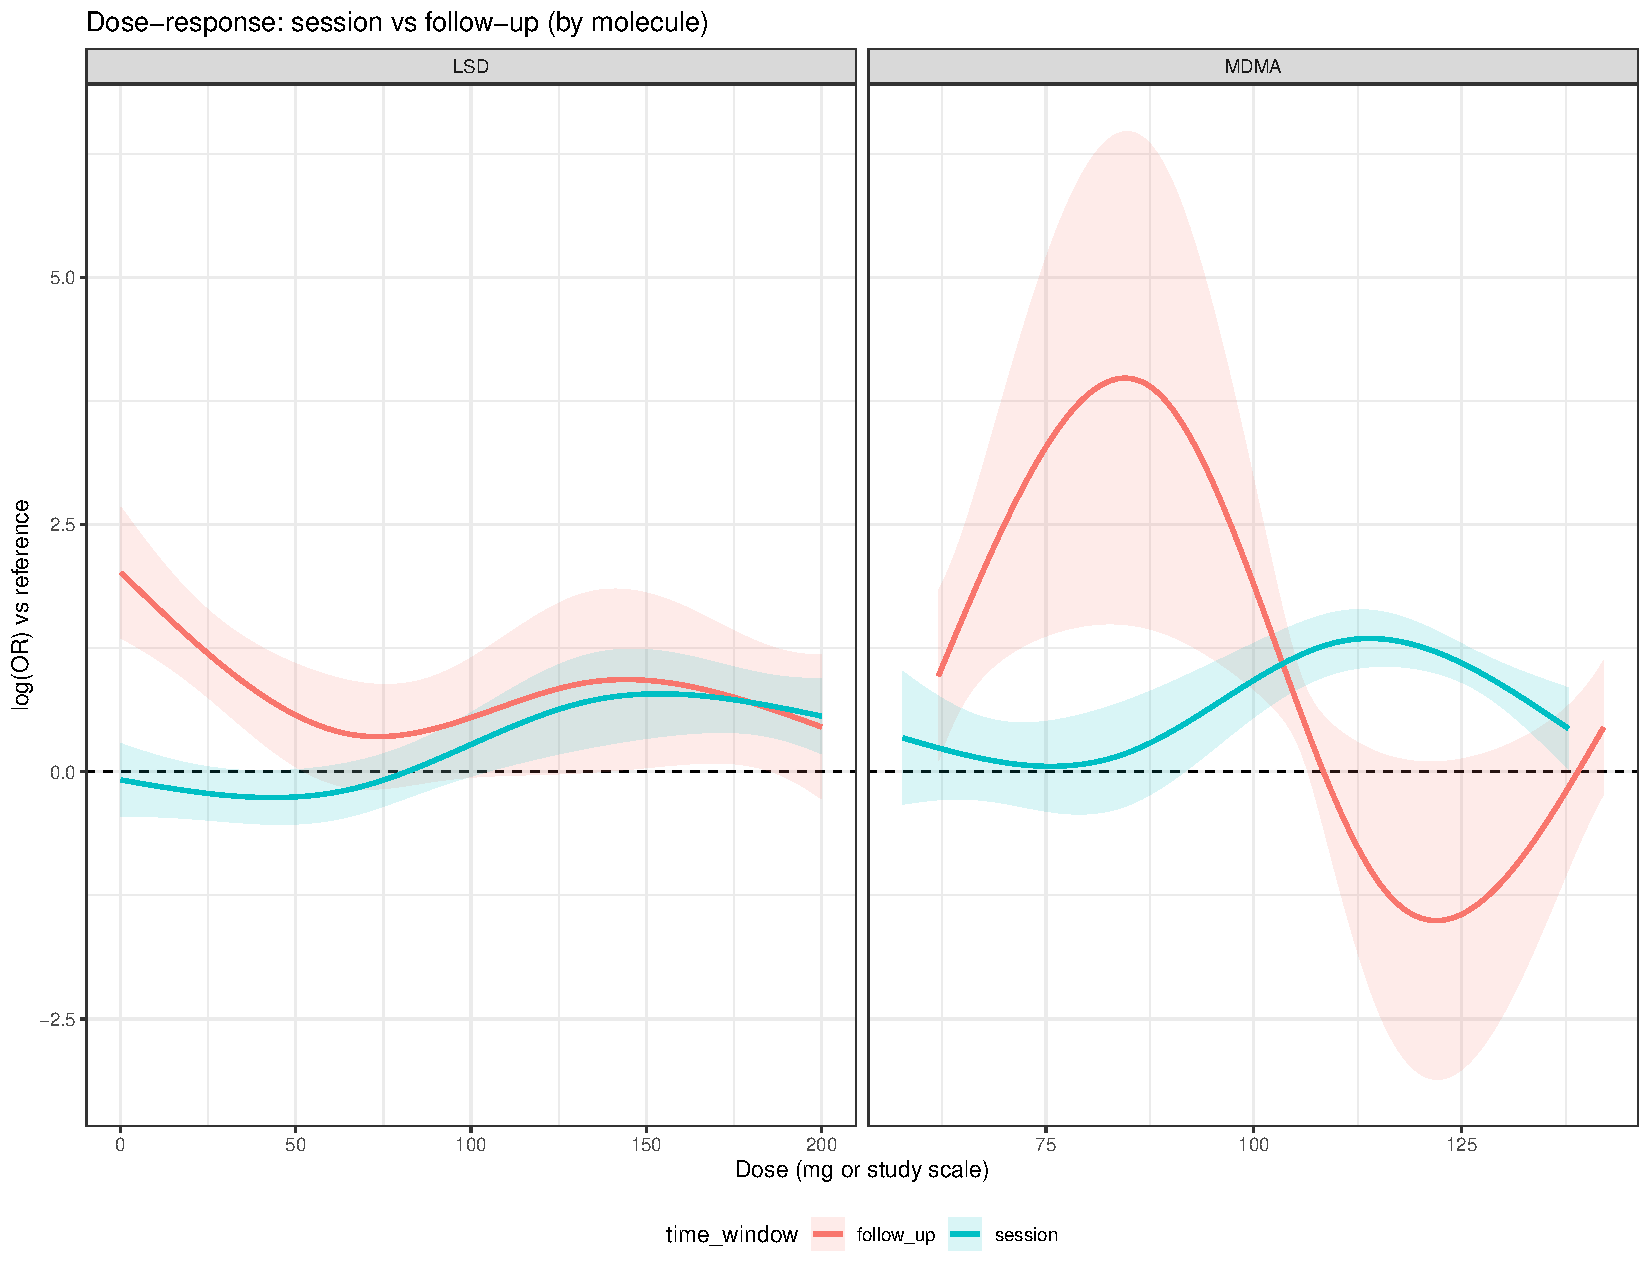
\includegraphics[width=0.94\textwidth]{figures/dr_session_vs_followup.pdf}
  \caption{\textbf{Global dose–response at session vs.\ follow-up (molecules with longitudinal data).}
  Modeled curves for LSD and MDMA by time window.}
  \label{fig:dr-session-followup}
\end{figure}


\subsection{Forest plots of AE incidence (drug vs.\ placebo) by time window}

\paragraph{Combined panel and molecule-level summaries.}
Figure~\ref{fig:forest-combined} shows a single combined panel of forest plots (one subpanel per molecule), with separate markers for the session and (where available) follow-up windows. This complements the dose–response view by addressing the categorical question: \emph{is a given AE significantly more frequent on drug than placebo in that window?} For LSD and MDMA, we further summarize which AEs are \emph{transient} (session-only), \emph{emergent} (follow-up-only), or \emph{persistent} (significant in both windows) using the transition table derived from the same models (Table~\ref{tab:ae-transition}).

\begin{figure}[htb]
  \centering
  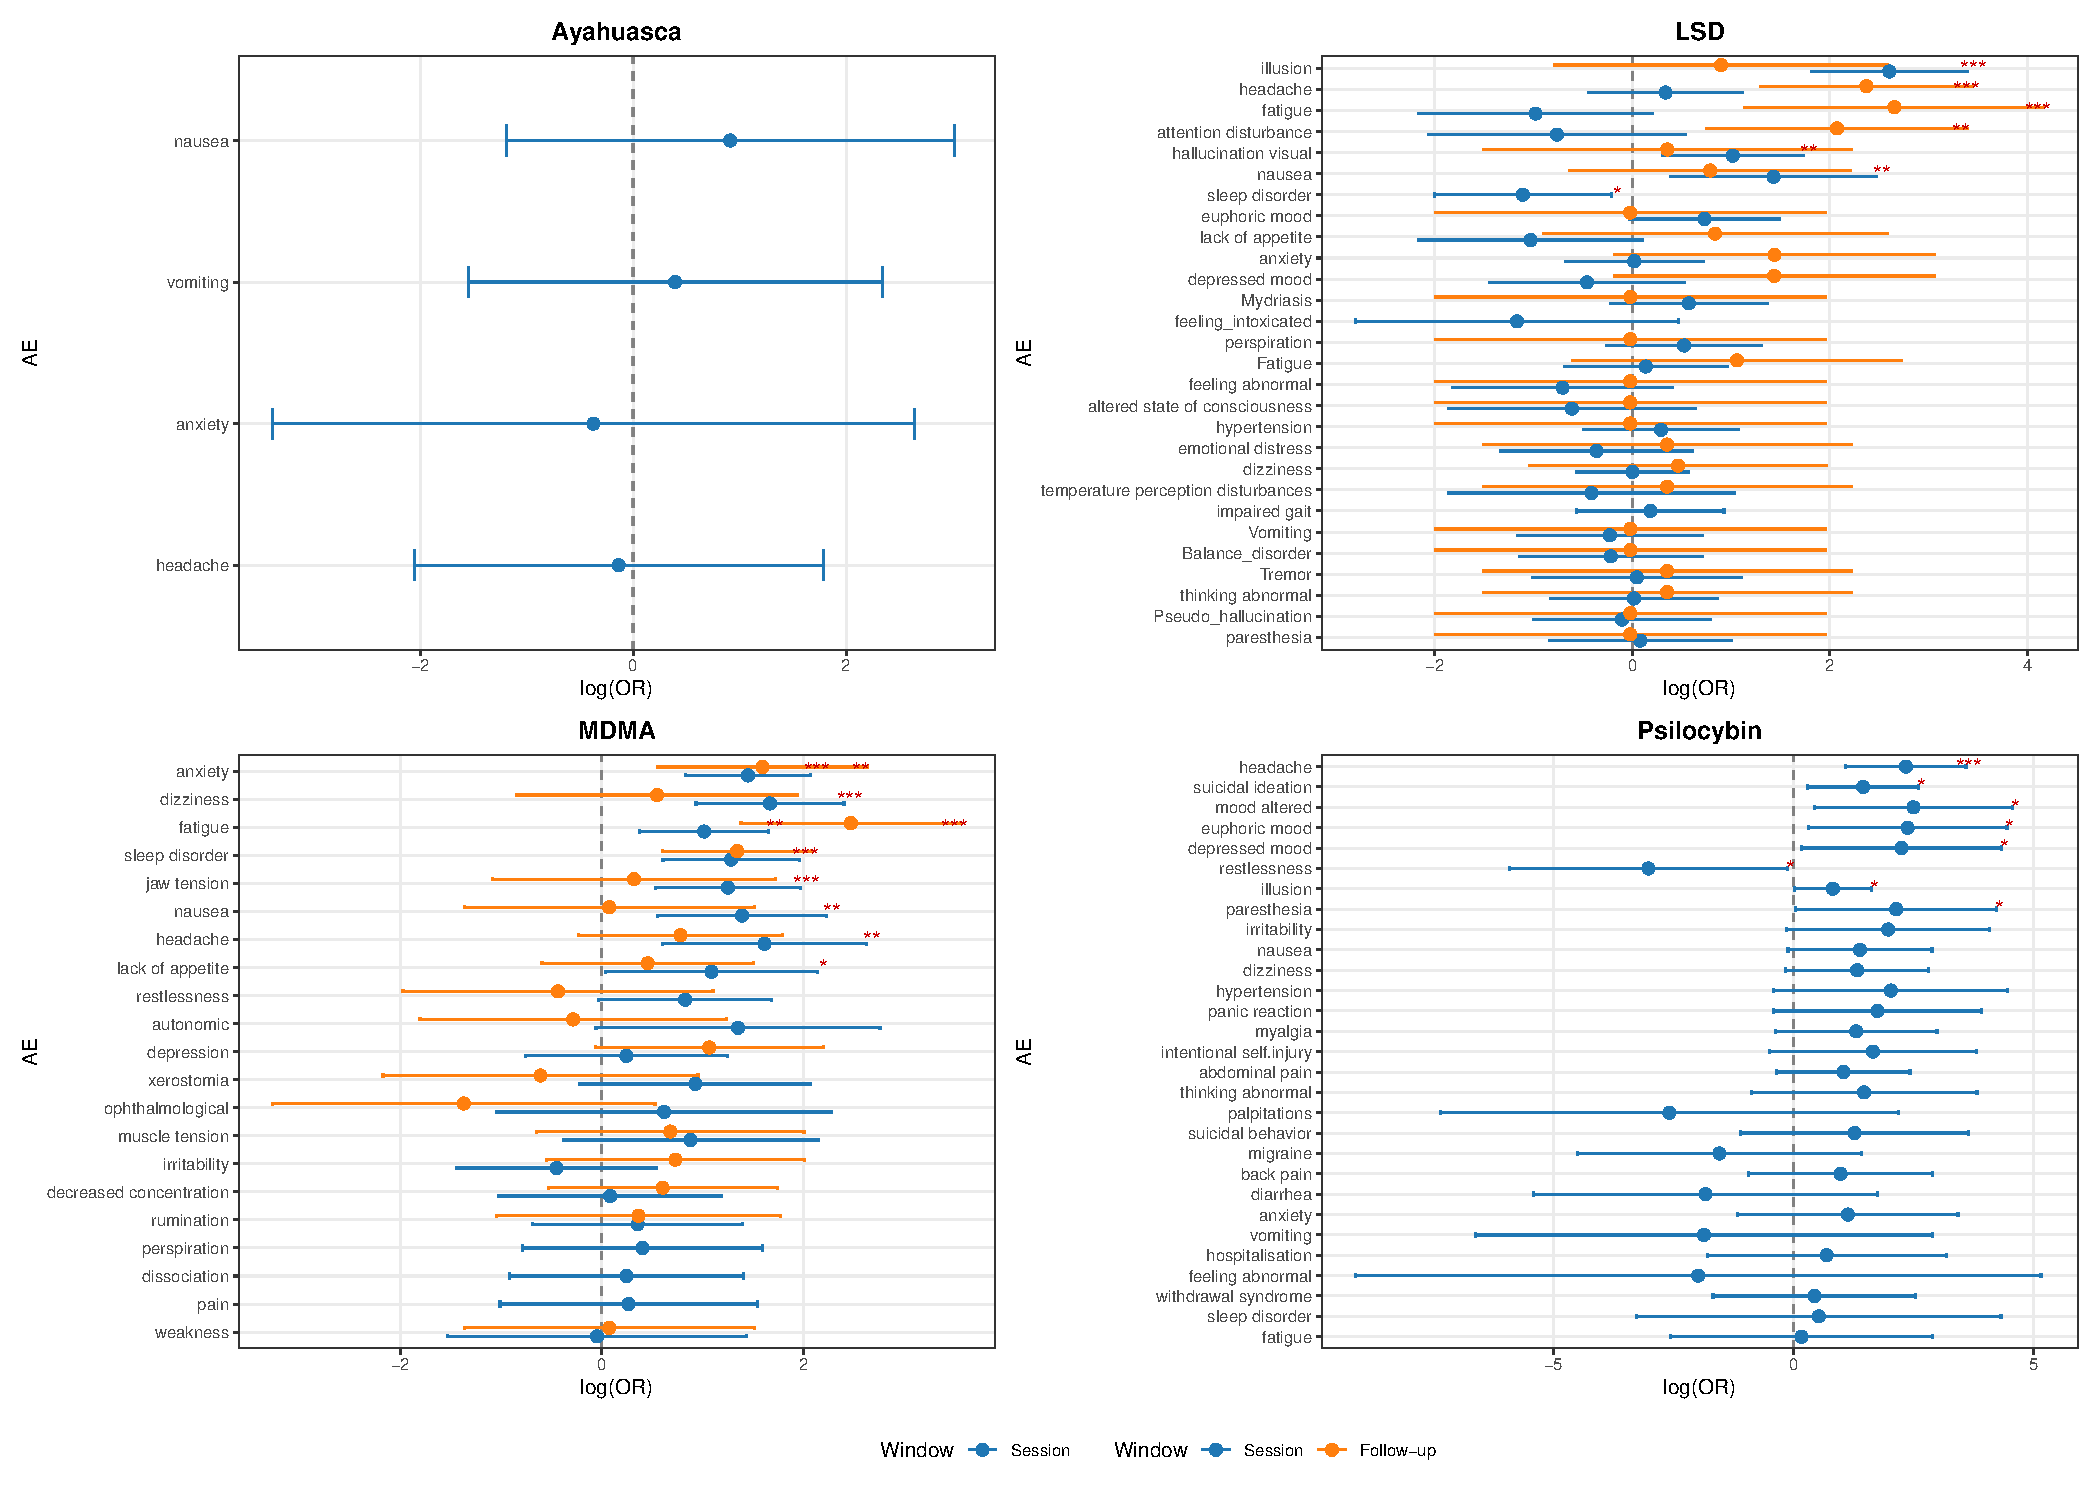
\includegraphics[width=0.98\textwidth]{figures/forest_combined_all_molecules.pdf}
  \caption{\textbf{Forest plots of AE odds ratios by molecule and time window.}
  Each subpanel lists AEs (rows) with pooled ORs (session and, if available, follow-up) vs.\ placebo; red highlights in the original graphics indicate p\,$<\,$0.05.}
  \label{fig:forest-combined}
\end{figure}


\begin{table}[!h]
\centering
\caption{\label{tab:ae-transition}
\textbf{Temporal status of significant adverse events (AEs) by molecule.}
AEs are classified as Transient (session-only), Emergent (follow-up-only), or Persistent (present in both windows).}
\resizebox{\textwidth}{!}{%
\begin{tabular}{llll}
\toprule
\textbf{Molecule} & \textbf{Transient (session-only)} & \textbf{Emergent (follow-up-only)} & \textbf{Persistent} \\
\midrule
LSD & hallucination visual; illusion; nausea; sleep disorder & attention disturbance; fatigue; headache & None \\
MDMA & dizziness; headache; jaw tension; lack of appetite; nausea & None & anxiety; fatigue; sleep disorder \\
PSILOCYBIN & depressed mood; euphoric mood; headache; illusion; mood altered; paresthesia; restlessness; suicidal ideation & None & None \\
\bottomrule
\end{tabular}
}
\end{table}


\paragraph{AE incidence by time window.}
Table~\ref{tab:ae-transition} and Figure~\ref{fig:forest-combined} summarize how adverse events (AEs) evolve between the acute \textit{session} phase and the \textit{follow-up} period.  
Overall, the majority of AEs across compounds were \textbf{transient}, occurring only during the drug session and resolving by the next assessment.  
Across all molecules, we identified \textbf{14 transient}, \textbf{5 emergent}, and only \textbf{3 persistent} AEs (Table~\ref{tab:ae-transition}).  

For \textbf{LSD}, the acute session was marked by four significant transient AEs --- \textit{visual hallucination} ($p<0.001$), \textit{illusion} ($p=0.002$), \textit{nausea} ($p=0.01$), and \textit{sleep disorder} ($p=0.03$) --- all of which resolved entirely by follow-up. Three emergent AEs appeared post-session: \textit{attention disturbance} ($p=0.04$), \textit{fatigue} ($p=0.01$), and \textit{headache} ($p=0.02$).  
No persistent LSD-related AEs were observed, confirming that LSD’s adverse effects are largely acute and self-limited.

For \textbf{MDMA}, a different pattern emerged. Five session-phase AEs were significant (\textit{dizziness} $p=0.02$, \textit{headache} $p<0.01$, \textit{jaw tension} $p<0.001$, \textit{lack of appetite} $p=0.04$, and \textit{nausea} $p<0.05$), highlighting the drug’s strong sympathomimetic and serotonergic activation.  
While these effects diminished after the session, three additional AEs became significant only at follow-up --- most notably \textit{fatigue} ($p<0.01$), \textit{sleep disturbance} ($p=0.03$), and \textit{anxiety} ($p<0.001$) --- suggesting delayed “comedown” phenomena.  
Importantly, three MDMA AEs (\textit{anxiety}, \textit{fatigue}, and \textit{sleep disorder}) remained significant in both windows, qualifying as \textbf{persistent} side effects that bridged the acute and post-acute phases.  
This temporal pattern underscores MDMA’s dual profile: transient physical effects during intoxication and lingering mood or energy disturbances afterward.

For \textbf{psilocybin}, seven AEs reached significance during the session: \textit{depressed mood}, \textit{euphoric mood}, \textit{headache}, \textit{illusion}, \textit{mood alteration}, \textit{paresthesia}, and \textit{restlessness} (all $p<0.05$).  
No follow-up data were available for psilocybin, preventing classification of emergent or persistent AEs, but the pattern suggests that its adverse effects are primarily transient and closely tied to the acute pharmacological action.

Finally, \textbf{ayahuasca} showed no statistically significant AEs after correction for multiple comparisons, likely reflecting the limited sample size and narrow dosing range. Nevertheless, trends toward gastrointestinal reactions (nausea, vomiting) were evident in raw incidence rates, consistent with the known pharmacological profile of the brew.

In summary, the temporal distribution of significant AEs reveals that LSD and psilocybin primarily induce short-lived, session-bound effects, whereas MDMA uniquely exhibits both transient physiological and delayed psychological adverse events.  
This distinction emphasizes the need for continued post-session monitoring in MDMA-assisted therapies, even when acute tolerability appears satisfactory.


\subsection{Why dose–response AE significance and forest (OR) significance may differ}

It is common for a given AE to be \emph{dose-sensitive} in the session (significant non-intercept dose term) yet not appear strongly significant in the pooled drug-vs-placebo comparison, and vice versa. Three practical mechanisms explain these discrepancies:

\begin{enumerate}
  \item \textbf{Threshold vs.\ gradient effects.} Some AEs turn on at low–moderate doses (so drug\,>\,placebo overall), but additional dose increases do not raise their frequency much; these yield significant forest ORs without a pronounced dose gradient.
  \item \textbf{High-dose concentration.} Other AEs occur mainly at the top dose(s). The dose–response test detects the gradient, but when all doses are pooled together, the overall drug\,vs\,placebo contrast is diluted by the low-dose arms and may not reach significance.
  \item \textbf{Window specificity.} Dose sensitivity can be visible in one window (e.g., session) while the categorical drug effect is stronger in another (e.g., follow-up). Comparing session vs.\ follow-up curves (Fig.~\ref{fig:dr-session-followup}) with forest ORs (Fig.~\ref{fig:forest-combined}) helps localize such timing effects.
\end{enumerate}

In practice, both views are complementary: dose–response tells \emph{how risk scales with dose}; forest ORs tell \emph{whether risk is elevated on drug vs.\ placebo in a given window}. We therefore report both throughout.
